\chapter{Cosmology basics} \label{ch:basics}

\section{Flat and curved spaces}
Cosmology is the study of the universe on the large scales, so we need to spend some time understanding how we are going to quantify and label positions in space and time.  Already in physics, we are used to labeling points in space with coordinates like $(x,y,z)$ or $(r,\theta,\phi)$.  We are also accustomed to computing the distances between points, especially in cartesian coordinates.

We know that the distance between two points can be computed from the coordinate differences via
\begin{equation}
  \Delta \ell = \sqrt{(\Delta x)^2 + (\Delta y)^2 + (\Delta z)^2 }.
\end{equation}
For infinitesimally small changes in the coordinates, we could write $  (d\ell)^2 = (dx)^2 + (dy)^2 + (dz)^2$, and use that to figure our the length of a curved path.  That equation is called the \textit{line element}\index{line element} and expresses the \textit{metric}\index{metric} of the space: it tells us how to measure distance.  For example, if a path traces out coordinates $x(\lambda),y(\lambda),z(\lambda)$ as a function of some parameter $\lambda$, we can measure the length with the integral
\begin{equation}
   \ell = \int_{\lambda_{\rm start}}^{\lambda_{\rm finish}} d\lambda \sqrt{ \left(\frac{dx}{d\lambda} \right)^2 + \left(\frac{dy}{d\lambda}\right)^2 + \left(\frac{dz}{d\lambda}\right)^2}.
\end{equation}
We recognize that this is the proper integral to use whether or not we are actually trying to evaluate it.

We also could change the coordinates that we use to define the space and trace out any given path.  For example, a Euclidean space in spherical polar coordinates has a metric
\begin{equation}
   d\ell^2 = dr^2 + r^2 d\theta^2 + r^2 \sin^2 \theta d\phi^2.
\end{equation}

We learn in special relativity that we need also to label event with space and time coordinates $(t,x,y,z)$, which is simple enough.  The surprise is that we further learn that different observers will disagree on the measurements of distances and time intervals, but all observers will agree on the spacetime interval between two events.  It is invariant.  The spacetime interval could be written as
\begin{equation}
  (\Delta s)^2 = -(\Delta t)^2 +  (\Delta x)^2 + (\Delta y)^2 + (\Delta z)^2
\end{equation}
for a straight path, or we could integrate along a curved path as with length before, treating time $t(\lambda)$ also as one of the parameterized coordinates.  The negative sign on time is a little weird but at least the space follows the familiar rules of Euclidean geometry.  The relationship between the three space coordinates, the one time coordinate, and the spacetime interval is called the spacetime metric.  The time coordinate $t$ is the wristwatch time of an observer but will not synchronize with the wristwatch time $t'$ of an observer in a different frame, one that moves with nonzero constant relative velocity.  We are going to measure time in units of length so that the units of the equation work out, thus taking the speed of light $c=1$.  For example, a time interval of $\Delta t = 1\,\mbox{m} = 1\,\mbox{m}/c = 3.3\times10^{-9} s$.

Our footing gets much less steady when we turn to general relativity, which is needed to treat accelerations and provides our best understanding of the physics of gravity, or to curved spaces.  In general, the space does not need to be Euclidean, so several of our common rules, such as ``the sum of angles in a triangle is $180^\circ$,'' might not hold.  Further, the numbers that we assign as coordinates to points in space are just labels, and (within some limits) we have enormous freedom to choose how we assign the coordinates.  (Some choices are easier to deal with than others.)  Like in special relativity, the spacetime interval along a path in the spacetime is invariant.

\begin{figure}[t]
  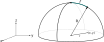
\includegraphics[width=\textwidth]{figs/basics/2d_spherical_surface.pdf}
  \caption{Diagram of a 2-d spherical surface embedded in 3-d cartesian coordinates.  The radius of the sphere is capital $R$, while the cylindrical distance from the 3-d origin to the point $(x,y)$ in the midplane is $r$.  The distance $\ell_{\rm radial}$ is the distance in the surface from a point to the 2-d origin at the north pole, while  $\ell_{\rm circumference}$ is the distance around.}\label{fig:2d_spherical_surface}
\end{figure}

We don't even need to get relativity to get experience with coordinates in curved spaces.  We can describe in polar coordinates the 2-d surface of the sphere (Figure~\ref{fig:2d_spherical_surface}), a surface in cartesian coordinates with equation $x^2 + y^2 + z^2 = R^2$.  Then $R$ is the radius of the sphere, and we let $r$ be the cylindrical distance from polar axis to a point on the sphere and $\phi$ be the azimuthal angle of that point to the $x$-axis.  It is not too much trouble to show that the length of a path along the surface from the north pole to a point is 
\begin{equation}
  \ell_{\rm radial} = \int_0^r \frac{dr'}{\sqrt{1-r'^2/R^2}} = R \sin^{-1}(r/R) > r. \label{eqn:2d_sphere_path_radius}
\end{equation}
So confined to the space (i.e.\ the surface), $r$ is the coordinate that labels the position away from the origin but is not the physical distance $\ell_{\rm radial}$ from the origin, which is larger.
We can also consider a circular path (all in the surface) with a fixed radius around the whole sphere, which has length,
\begin{equation}
  \ell_{\rm circumference} = \int_0^{2\pi} d\phi r = 2\pi r.  \label{eqn:2d_sphere_path_circumference}
\end{equation}
So that circle, considered along the curved surface only, has more radius than you would expect given the circumference.  This is a manifestation of the surfaces positive curvature.  Also note that that point with $r=0$ is not a special point of the sphere.  All points are the same because, mathematically, a sphere is homogeneous and isotropic, so we could have defined that origin point anywhere. From Eqns. (\ref{eqn:2d_sphere_path_radius}) and (\ref{eqn:2d_sphere_path_circumference}) we can work out that the metric for the surface of the sphere is,
\begin{equation}
  d\ell^2 = \frac{1}{1-r^2/R^2} dr^2 + r^2 d\phi^2.
\end{equation}
A sphere with a very large radius $R$ compare to the coordinate $r$ values of interest looks pretty flat, and that is reflected in the metric.  When we get to cosmological metrics in the next pages, the present-day cylindrical radius $r$ to a point will correspond to the comoving radial coordinate, while the distance in the space $\ell$ will correspond to the comoving distance (usually given the symbol $\chi$).

For a 2-d hyperbolic surface that satisfies $x^2 + y^2 - z^2 = R^2$, the metric is similar, differing only in the sign of the addition in the denominator of the radial term,
\begin{equation}
    d\ell^2 = \frac{1}{1+r^2/R^2} dr^2 + r^2 d\phi^2.
\end{equation}
It is also a homogeneous and isotropic space, but has less radius than you would expect for a given circumference, compare to a flat plane.

Both these spherical and hyperbolic surfaces are two-dimensional surfaces that we have embedded in three-dimensional Euclidean space.  We can go to one higher dimension, looking at 3-d surfaces that satisfy $x^2 + y^2 + z^2 \pm u^2 = R^2$.  These spaces work basically the same and we unsurprisingly find a spherical-polar metric with,
\begin{equation}
  d\ell^2 =  \frac{1}{1-kr^2/R^2} dr^2 + r^2 d\Omega^2,
\end{equation}
where the solid angle $d\Omega^2 = d\theta^2 + \sin^2 \theta d\phi^2$, and the parameter $k$ is $+1$ for a spherical space and $-1$ for a hyperbolic space.  We can also include the value $k=0$ to recover normal 3-d spherical polar coordinates.  Notice that all of the metric weirdness is in the radial coordinate.  The angular part of the metric looks pretty normal, so the  radius of a circle is still $2\pi r$ and the surface area of a sphere is still $4\pi r^2$, but you have to be a little careful about what you mean by $r$, because, except in flat space, it is not the physical distance from the origin.

\section{Cosmological FRW metric}
For much of practical observational cosmology, we will not need much general relativity, but a few results are crucial.  As noted before, we observe that the universe is statistically homogeneous and isotropic, meaning that at different locations and in different directions, the universe is basically the same: composed of galaxies of the same various types, oriented in all different directions at random.  It is also true is that the universe is not static, but dynamic; it changes in time.  When we look at the most distant galaxies, where the light has taken many billions of years to reach us, the galaxies are different, forming stars alternatively less then more then less vigorously.  Older galaxies have more pristine gas with fewer heavy elements.  Moreover, the light from distant galaxies is \textit{redshifted}\index{redshift}, or shifted to longer wavelengths, which is strong evidence that the universe is expanding in time, as we will see.

In general relativity, these conditions end up being very restrictive.  The metric that describes how to measure spacetime intervals in homogeneous, isotropic, dynamic spacetimes are limited to ones written as
\begin{equation}
  ds^2 = -dt^2 + a^2(t)\left[ \frac{dr^2}{1 - kr^2/R_0^2} + r^2 d\Omega^2  \right]
\end{equation}
where $r$ is a radial coordinate (called a comoving coordinate) but again is slightly different to what we are used to, and $\theta$ and $\phi$ are angular coordinates that work normally.  This metric is extremely important.  The parameter $k$ denotes the three different kinds of spacetimes that are allowed by our restrictive conditions.  Values $k = \{ -1, 0, +1 \}$ mean that the space has negative curvature, is spatially flat, or has positive curvature.    All of this is familiar from our discussion of curved spaces above.

The new element is the function $a(t)$, which is called the \textit{scale factor}\index{scale factor} and specifies how the size of the universe changes over time.  By convention, we set $a(t_{\rm now}) = 1$, which means that the comoving coordinate refers to the present time. Similarly, the parameter $R_0 > 0$ is the radius of the curvature of the space at the present day, but the curvature scale at other times grows or shrinks according to $a(t)$.  The meaning of $t$ is the wristwatch time of ``co-moving'' observers.  By comoving, we mean these are observers who are carried along with the expansion of the universe.  Their coordinates $(r,\theta,\phi)$ are fixed and their relative motions are determined only by the expansion.  They have no independent motion (that is, peculiar velocity\index{peculiar velocity}).

We call this metric the Friedmann-Robertson-Walker (FRW) or Friedmann-Lemaitre-Robertson-Walker (FLRW) metric after the people who found and worked with it first.  We have measured the spatial curvature and know that the radius of curvature exceeds $R_0 > 60$\ Gpc (at 95\% confidence in Planck satellite data), so our universe is fairly flat.  In some instances, we will restrict to that flat case.  Cosmology is concerned with the very largest size scales in the universe.  We are essentially stuck in one spot, in the Milky Way, so we can call our position as the origin of our coordinate system, $r=0$. 

The expansion rate at any time is given by the time derivative of the scale factor.  This is typically rescaled by the scale factor itself to give the \textit{Hubble parameter}\index{Hubble parameter},
\begin{equation}
  H = \frac{1}{a} \frac{da}{dt} = \frac{\dot a}{a}. 
\end{equation}
The present-day expansion rate is called the \textit{Hubble constant}\index{Hubble constant},
\begin{equation}
  H_0 = H(t_{\rm now}) = \frac{\dot a(t_{\rm now})}{1} \approx \frac{70\,\mbox{km/s}}{\mbox{Mpc}} \approx 2.3\times 10^{-18}\,\mbox{s}^{-1}.
\end{equation}
All determinations of distance depend on the Hubble constant; it is an enormously important quantity and there is still some few percent disagreement about its value.  The inverse of the Hubble constant can be expressed as a time, about 240 Myrs, or a distance, about 4.2 Gpc.
  
In flat space ($k=0$), the physical distance (like you would measure with a ruler) from the origin to a point depends on the comoving coordinate as
\begin{equation}   
  \ell_{\rm radial} = a(t) r 
\end{equation}
while the physical velocity of an object is
\begin{equation}
  v_{\rm phys} = \frac{d(\ell_{\rm phys})}{dt} = \frac{da}{dt} r + a \frac{dr}{dt} = \frac{\dot a}{a} a r + a \frac{dr}{dt} = H \ell_{\rm phys} + v_{\rm pec}
\end{equation}
The first term in the velocity is called the \textit{Hubble flow}\index{Hubble flow} and the second term is called the \textit{peculiar velocity}\index{peculiar velocity}.  The Hubble flow is the velocity that you measure from the expansion of the Universe.  Nearby, where the Hubble parameter is close to the present-day value, we find that galaxies tend to move away from us at around 70 km/s per Mpc of distance away.  The peculiar velocity is the independent velocity of a galaxy and is typically around 1000 km/s, so we need to look further than tens of Mpc away for the Hubble flow to dominate the overall velocity of an object.  In practice, we measure the \textit{cosmological redshift}\index{redshift}, $z$, of the spectral lines of an object compared to the wavelength of emission.
\begin{equation} 
  \lambda_{\rm obs}/\lambda_{\rm em} = a(t_{\rm now}) / a(t_{\rm em}) = 1+z.
\end{equation}
We have $z=0$ at the present day, $z \sim 10$ when the first stars and galaxies are forming, and $z =1100$ when the CMB is released.  The wavelength is expanded, but since the speed of light is constant, the frequency of light slows, as does the observed rate of any other process.  Thus energy and momentum of photons (and other objects) drops as the Universe expands.

Does this violate conservation of energy?  Well, no, energy conservation is the result of the symmetry of time-invariance.  The spacetime of an expanding universe is not time invariant, so we cannot expect energy conservation.  As the momentum of objects redshifts away, they over time lose their peculiar velocities and come to join the Hubble flow.

\section{Friedmann equations and model universes}
Much of the development of the universe clearly depends on the \textit{expansion history}\index{expansion history}, the scale factor as a function of time: $a(t)$.  Treating the contents of the universe the as a uniform fluid, the Einstein differential equations of general relativity---which relate the curvature expressed by the metric to the matter-energy content---yield two differential equations that relate the scale factor to the energy density $\rho$ and pressure $P$ of the fluid. These equations are the first Friedmann equation,
\begin{equation}
  H^2 = \left( \frac{\dot a}{a} \right)^2 = \frac{8\pi G}{3} \rho - \frac{k}{a^2 R_0^2}, \label{eqn:friedmann1}
\end{equation}
and the second Friedmann equation,
\begin{equation}
  \frac{\ddot a}{a} = -\frac{4 \pi G}{3} (\rho + 3 P) \label{eqn:friedmann2}.
\end{equation}
Examining the first Friedmann equation we see that the expansion rate on the left and contributions from the density and the curvature on the right, while in the second Friedmann equation we see the acceleration of the scale factor on the left related to the density and pressure on the right.

\subsection{Components of the Universe}
We need to describe the types of matter and radiation in the Universe that contribute to the Friedmann equations.  We also need to understand how the densities change with the scale factor, which allows us to solve these differential equations for $a(t)$.  In relativity, we do not have energy conservation but we do have a continuity equation\index{continuity equation} that describes how matter and energy are transported through spacetime.   We don't develop the background here to derive it, but the result for a perfect fluid is,
\begin{equation}
  \dot \rho + 3 \frac{\ddot a}{a}(\rho + P) = 0.
\end{equation}
We often consider a proportional relationship between pressure and density, the \textit{equation of state}\index{equation of state} with equation of state parameter $w$ as the constant of proportionality,
\begin{equation}
  P = w \rho.
\end{equation}
This allows us to solve the continuity equation to relate density to the scale factor of expansion.
\begin{equation}
  \rho \propto a^{-3(1+w)}
\end{equation}
Let's see how that relates to various types of substances.

\paragraph{Matter.}  When we talk about \textit{matter}\index{matter}, we are referring to non-relativistic particles for which the kinetic energy is small compared to the rest mass and (equivalently) the pressure is small compared to the density ($P \ll \rho$ in units where $c=1$).  Thus $w=0$, and the continuity equation provides
\begin{equation}\rho \propto a^{-3}.\end{equation}
This result makes sense: density is diluted by the expansion to the third power.  The total density of matter is the particle rest mass times the number density, $\rho_m = mn$, and the number density of particles is diluted by the expansion of the universe as $n \propto a^{-3}$.

Our universe includes at least two categories of matter.  The normal matter\index{matter!normal} consist of the types that we are most familiar with on Earth: proton, neutrons, nuclei, atoms.  In the late universe, there are dense object like planets and stars, but even today the bulk of the normal matter is in the form of diffuse gas or plasma.  This component is also sometimes given the catchall term ``baryons.''  This component does have some pressure, which is important for driving acoustic oscillations in the CMB, but even at that time and ever since, the overwhelming majority of the baryons were non-relativistic, so the pressure was not important in determining their contribution to the expansion history.  Their contribution is dominated by their rest mass.

The second category of matter, \textit{dark matter}\index{matter!dark}, is a substance of unknown type that contributes about five times as much to the total density budget as normal matter.  It is unclear if this is a subatomic particle or something macroscopic.  We do not know if there is one type or multiple types that fill out an entire ``dark sector'' of particle physics.  There is so far no evidence for interactions between this component and photons or baryons, or with itself.  As such, this component seems to genuinely provide no pressure, and is usually modeled that way, although in actually there may be some interactions at very low level (which would be our main hope of discovering it in a particle physics detector).  Some models include weakly-interacting massive particles (WIMPs), axions (proposed particles to solve the strong CP problem in QCD), and primordial black holes.

\paragraph{Radiation.}  For photons or any gas of relativistic particle, the pressure relates to the energy density as
\begin{equation}
  P_r = \frac{1}{3} \rho_r
\end{equation}
or $w=1/3$.
This in turn means that the energy density scales with expansion as
\begin{equation}
  \rho_r \propto a^{-4}.
\end{equation}
The expansion of the volume dilutes the photon number density while the energy per photon is redshifting away, thus $\rho \propto n E \propto a^{-3}a^{-1}$.

Included in radiation are photons, light particles (including neutrinos), and gravitons.  The  photons are predominantly those that at late times becomes the CMB.  These photons follow a thermal (Planck) blackbody spectrum and the redshift effect is the same as adjusting the temperature $T \propto a^{-1}$.  Thus it makes sense to talk about a (radiation) temperature of the universe at various times.

What we count as a light particle depends on when in the history of the universe we are talking about.  A particle is relativistic ($\gamma \gg 1$) when its total $\gamma m$ is large compared to its rest mass $m$.  At early times, the total energy $E \sim kT$, and the temperature can be as high as the scale factor is small.  Thus every particle is relativisitic if you go back early enough in the course of the universe.  Radiation is the dominant contribution to the energy density early on.  Neutrinos are relativistic for the early history of the universe, and although we don't yet know all the neutrino masses, at least some neutrinos are massive enough to not be relativistic now.

Gravitons are massless particles and so are always relativistic, but they don't have much overall energy density and contribute negligably to the expansion history.

\paragraph{Dark Energy.}\index{dark energy}  In General Relativity, the Einstein equations are differential equations that relate the properties of spacetime on one side and matter-energy content on the other.  They are not uniquely determined and you can add a term proportional to the metric tensor without messing up the continuity equation for the stress-energy density.  Einstein originally introduced such a term, conventionally written as proportional to some constant number $\Lambda$, essentially asserting it as an innate property of spacetime.  He did this because it allows solutions to the equations that corresponded to the static universes he desired, ones unchanging in time.  (When the universe was later found to be expanding, Einstein famously called this added term his ``greatest blunder.'')

Another point of view is to consider what that term would mean if you moved it to the other side of the equation, mathematically equivalent, and considered it as a type of energy density.  It acts as a fluid with the equation of state
\begin{equation}
  P_\Lambda = -\rho_\Lambda,
\end{equation}
which has a positive energy density but a negative pressure.  The equation of state parameter is $w=-1$ and so
\begin{equation}
  \rho_\Lambda \propto a^0
\end{equation}
is constant.  The density of this component does not dilute with expansion of the universe.  This is very weird and  does not fit with our intuitions of how substances work.  However, current modeling requires this component, dubbed ``dark energy,'' to account for about 70 percent of our present-day energy budget.

This component is utterly mysterious to us.  It may ultimately be simply a property of spacetime as originally envisioned, just a \textit{cosmological constant} in the equations of GR.  It may be an energy density associated with the vacuum.  This might make the density dependence on expansion more understandable.  An expanding volume produces more vacuum and so produces more dark energy.  In quantum mechanics, the (observed) Casamir effect depends on a sea of vitual particles and a zero-point energy associated with the vacuum.  However, a simple theory computation, accounting for the particles we know about, predicts a vacuum energy value which is huge, a factor of $10^{60}$ greater than what we observe.  This is the unresolved \textit{cosmological constant problem}.

There are other models where the dark energy is one or more particle physics field and could be dynamic and not a constant after all.  Consistent with that, there may be some preliminary evidence that dark energy equation of state is not a constant at $w = -1$, but it's not yet totally clear.   This is an active area of research.

\subsection{Expansion histories of model universes}
With the $\rho(a)$ dependence of the of the different components, we can solve the Friedmann equations directly in simple cases.  For example, in flat universes that are dominated by a single component, we find for different equations of state that,
\begin{equation}
  a(t) \propto \left\{
  \begin{array}{lll}
    t^{2/3(1+w)}  = \left\{ \begin{array}{l} t^{2/3}\\ t^{1/2} \end{array} \right. & \begin{array}{l} w=0  \\ w = 1/3 \end{array} &  \begin{array}{l} \mbox{matter-dom.}  \\ \mbox{radiation-dom.} \end{array} \\
    \exp(Ht) & \begin{array}{l}w = -1 \end{array}& \begin{array}{l} \Lambda\mbox{-dom.} \end{array}
  \end{array}
  \right. 
\end{equation}
There are several things to note about these solutions.  The matter and radiation solutions are increasing in size but decelerating (concave-down curves), and we understand this in terms of the attractive gravitational pull of all the matter in the universe slowing the expansion.  In a flat universe, however, it is not enough to arrest the expansion.

In a flat, cosmological-constant-dominated Universe, by contrast, the expansion is exponentially accelerating.  The Hubble parameter is always constant in this case.   We think that our universe today has mostly transitioned from being matter dominated to dark-energy dominated, as the expansion dilutes the matter but not a cosmological constant.  The components had equal energy density about $z=0.3$.  The matter-dominated phase lasted about 10 Gyr.  Because of the density scaling with scale factor, prior to the matter dominated phase was a radiation dominated phase (equal densities about $z=3400$).  The radiation dominated phases lasted only about 50 kyr.  Looking backward in time, both matter- and radiation-dominated universes reach zero size a finite time in the past.  This is the origin of the idea of the ``hot Big Bang.''  We additionally think there was another, earlier epoch of exponential expansion prior to the radiation dominated phase.  This is \textit{inflation}\index{inflation} and we understand that even less than dark energy.  We'll talk about it more when we discuss the cosmic microwave background.

Because our Universe has multiple components, and curvature is always a possibility, we need to treat the solution for $a(t)$ more generally.  From the first Friedmann equation (\ref{eqn:friedmann1}), we see that for a particular expansion rate there is a particular \textit{critical density}\index{critical density} associated with flatness.  To have a flat ($k=0$) universe today ($a=1$, $H=H_0$), we must have
%\begin{equation}
%  H_0^2  = \frac{8\pi G}{3} \rho_{\rm crit,0} 
%\end{equation}
\begin{equation}
  \rho_{\rm crit,0}   = \frac{3 H_0^2}{8\pi G},
\end{equation}
a density that works out to be about one Milky Way-sized galaxy per cubic Mpc.  We do not see that much luminous matter, but the other components, dark matter and dark energy, make up the difference, leaving our Universe very close to flat.

We can cast the first Friedmann equation into a nice form by looking at the ratio of the density to the critical density for each component
\begin{equation}
  \Omega_i = \frac{\rho_{i,0}}{\rho_{\rm crit,0}}
\end{equation}
for $\Omega_r$, $\Omega_m$, and $\Omega_\Lambda$.
We can define an analogous quantity for curvature, 
\begin{equation}
  \Omega_k = \frac{-k/R_0^2}{H_0^2}   \qquad \mbox{or} \qquad R_0 = \frac{1}{H_0\sqrt{-\Omega_k / k}},
\end{equation}
but note the change in sign, so that $\Omega_k<0$ for positive curvature $k>0$.  With current limits on $|\Omega_k| < 0.005$, we know that $R_0 > 60$ Gpc.   With these, the Friedmann equation \ref{eqn:friedmann1} becomes,
\begin{equation}
  H(a)^2 = H_0^2 ( \Omega_r a^{-4} + \Omega_m a^{-3} + \Omega_k  a^{-2}+  \Omega_\Lambda ) = [ H_0 E(a) ]^2. \label{eqn:H_in_terms_of_Omega}
\end{equation}
Note that for $a=1$, this form shows that the sum of the $\Omega$ parameters is unity, and while $\Omega_k$ (and potentially $\Omega_\Lambda$ but not in actuality) could be negative, the others can only be positive.  Rearranging, we get a separable equation
\begin{equation}
\frac{da}{dt} = \dot a = H_0 (\Omega_r a^{-2} + \Omega_m a^{-1} + \Omega_k  +  \Omega_\Lambda a^2)^{1/2} = H_0 F(a), \label{eqn:friedmann_adot}
\end{equation}
that can be integrated and inverted to give the functional relationship between $a$ and $t$,
\begin{equation}
  \int^1_a \frac{da'}{H_0 F(a')} =  \int^{t_{\rm now}}_t dt'.
\end{equation}
Many of the two-component universes have analytic solutions, but our $\Lambda$CDM universe needs to be numerically integrated and it is trivial to do so to whatever accuracy we require.


\begin{figure}[t]
  \begin{center}
    \includegraphics[width=\textwidth]{figs/basics/a_of_t.pdf}
  \end{center}
  \caption{For the $\Lambda$CDM model and several others, the scale factor $a(t)$. and $H(t)$, with $z$ on the other axis.  All models have the same scale factor and slope (Hubble constant) at the present day, $t-t_{\rm now} = 0$.
    The $\Lambda$CDM  model that fits well our own universe takes a longer time to develop compared to the others, a consequence of the low matter density and late-time, cosmological-constant-driven accelerated expansion.  For the other model universes are younger.  The stronger gravity of a higher matter density causes more rapid deceleration to the present day values of the slope of the expansion. The flat, matter-dominated universe grows as $a \propto t^{2/3}$, as we saw before.
  }\label{fig:a_of_t}
\end{figure}
In broad terms, the expansion of the spacetime of our universe fits a model with roughly $\Omega_m=0.3$, $\Omega_\Lambda=0.7$, and no spatial curvature $\Omega_k=0.0$ that is currently expanding with $H_0 \sim 70$ km/s/Mpc.  This is illustrated in Figure~\ref{fig:a_of_t} with a few other models.  The scale factor in these models goes to zero in the finite past, which gives the age of the universe and the epoch of the Big Bang\index{Big Bang}.

Looking at Equation \ref{eqn:friedmann_adot}, as $a$ increases, we can work out that these particular open and flat models will expand forever.  The flat $\Lambda$CDM model reaches exponential expansion in the far future.  The open, low-matter and flat, matter-dominated are constantly decelerating (Figure \ref{fig:expansion_rate}), with the open model achieving constant positive $\dot a = H_0\Omega_k^{1/2}$ after infinite time and the flat, matter-dominated universe approaching $\dot a \rightarrow 0$ after infinite time.  The high matter universe with positive curvature is different in that the gravitational pull of the matter is sufficient to stop the expansion and recollapse the universe to zero scale factor in finite time, a so-called ``Big Crunch.''\index{Big Crunch}  Such a symmetric fate for the Universe, particularly paired with the notion of a recurring cycle of Big Bangs and Big Crunches is philosophically appealing, but the data appear to have ruled it out.

\begin{figure}[t]
  \begin{center}
    \includegraphics[width=\textwidth]{figs/basics/expansion_rate.pdf}
  \end{center}
  \caption{The expansion rate for several models.  Notably, the $\Lambda$CDM model has an expansion rate that decreases when matter is dominating and then increases again as the dark energy begins to affect the dynamics.  The expansion of the universe decelerates, then accelerates.  The other models show only deceleration.  The expansion rate is much higher in the early history of the universe.  The radiation dominated epoch is only a few ten thousand years and is not visible on a plot like this.} \label{fig:expansion_rate}
  \end{figure}


These ``$\Omega$'' parameters are the first of what we will call \textit{cosmological parameters}\index{cosmological parameters}.  They determine how a specific cosmological model develops over time.  Much of the science of observational cosmology is dedicated to making measurements of observable quantities and using them to determine the values of the cosmological parameters within a particular model.






\section{Distance measures}

The redshift of objects is an observable that is relatively easy to measure, directly provides the amount of expansion in the universe since that time, and gives us one notion of the distance to an object.  We need to understand the relationship between redshift and the other observables that are also related to distance, most prominently the brightness and angular size of objects.  Brightness and angular size are also relatively easy to measure on the sky.  Comparisons of these observables and their associated distance--redshift relationships over cosmic time give us useful ways to constrain the cosmological model.

Important in the discussion of distances are the concepts of \textit{standard candles}\index{standard candle} and \textit{standard rulers}\index{standard ruler}.  A standard candle is an object of known luminosity that we can compare to its measured brightness to determine the distance.  The most well-known standard candles are type Ia supernova, exploding white dwarf stars.  These are sometimes referred to as ``standardizable candles'' since they are not all identical, and their luminosity is not known from first principles, but the luminosity can be well calibrated by a series of observations that we will describe in chapter \ref{ch:standard_candles}.  A related concept is a standard siren\index{standard siren}, which is a gravitational wave source of known power that we can compare to the locally measured strain.  An example would be a binary black hole merger that is (1) understood in such detail that the power is understood and is (2) localized such that the redshift of the host galaxy is measureable.

A standard ruler is an object or feature of known comoving or physical size that we can compare to the measured angular size.  Examples of standard rulers are the baryon acoustic oscillations---soundwaves in the primordial plasma---that are visible both as peaks in the CMB power spectrum and in the distribution of galaxies.  

If we want to work out the distance to a point where some radiation was emitted, we can integrate
\begin{equation}
  d\chi = \frac{dr}{(1 + kr^2/R_0^2)^{1/2}}
\end{equation}
along the radial path to the point, similar to when we integrated $d\ell$ on the surface of the sphere.  In a similar way, we get, 
\begin{equation}
  r = S_k(\chi) \equiv \left\{
  \begin{array}{ll}
    R_0 \sinh(\chi/R_0) &  k=-1; \\
    \chi & k=0; \\
    R_0 \sin(\chi/R_0) &  k=+1.
  \end{array}
  \right.
\end{equation}
You can compare Equation~(\ref{eqn:2d_sphere_path_radius}) to see that $\chi$ is the radial distance in the (possibly) curved space.  We do this all at the present day, when $a=1$.  We call $\chi$ the comoving distance\index{comoving distance}.

Writing the FRW metric in terms of the comoving distance, we have
\begin{equation}
  ds^2 = -dt^2 + a^2 \left[ d\chi^2 + S_k^2(\chi) d\Omega^2 \right].
\end{equation}
Photons travel on null geodesics, paths with $ds^2 = 0$, so a photon on a radial path ($d\theta = d\phi = 0$) will have
\begin{equation}
  d\chi = \frac{dt}{a(t)} = - \frac{dz}{H(z)}
\end{equation}
where we have used the differential of $1+z = 1/a(t)$ in the last equality.  Integrating, we find
\begin{equation}
  \chi = \int_{t_{\rm em}}^{t_{\rm now}} \frac{dt}{a(t)} = \int_0^z \frac{dz'}{H(z')}  = \frac{1}{H_0} \int_0^z \frac{dz'}{E(z')} \label{eqn:chi_of_z}
\end{equation}
to get $\chi(t)$ or more usefully $\chi(z)$. As we see, this distance--redshift relation measures expansion history via the integrated $1/a(t)$ or $1/H(z)$.  Comparing Equation~(\ref{eqn:H_in_terms_of_Omega}), you can see that $\chi(z)$ has an amplitude determined by $H_0^{-1}$ and a shape determined by the the $\Omega$ parameters (i.e.\ the composition of the Universe).

This discussion has readied us to examine several additional, distinct notions of cosmological distance.

\begin{figure}[!t]
  \begin{center}
    {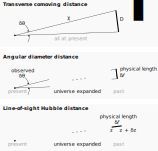
\includegraphics[width=\textwidth]{figs/basics/DM_DA_DH_diagram.pdf}}
  \end{center}
  \caption{Diagrams that help explain cosmological distance measures.  The transverse comoving distance is based of an arc drawn at the present day, so the expansion of the universe doesn't affect it. In a flat geometry, $D_M = \chi$ and this is exactly the familiar relation.   The angular diameter distance helps us account for the size that physical length will expand into.  The Line-of-sight comoving Hubble distance accounts for the expansion of the universe as light travels from the far side to the near side of an object.
}
  \label{fig:distances1}
\end{figure}


\paragraph{Comoving distance.}
As mentioned, we call $\chi$ the comoving distance.  It is the physical distance today if we were to measure with a ruler to the point where the emission (previously) came from.

\paragraph{Transverse comoving distance.}  This also sometimes called the metric distance and people often use the symbol $D_M$.  This is the distance used to compute an arc length \textit{as measured today}, so we are not worried about the expansion of the universe.  So an arc with angle $\delta\theta$ and radius $\chi$ has an arc length $D_M \delta\theta$.  See Figure~\ref{fig:distances1}.  We have already encountered this quantity, which has the value
\begin{equation}
  D_M(z) = S_k(\chi(z)) = r(z).
\end{equation}
finding that it is the same value as the comoving coordinate.  In a flat universe only, this quantity is also the comoving distance $\chi$.

\paragraph{Angular diameter distance.}  Suppose an object with physical size $\delta\ell$, a standard ruler perpendicular to the line of sight, emitted radiation in the past at redshift $1+z = 1/a$.  Today it  subtends angle $\delta\theta$.
We just saw how to relate the comoving (present-day) arc length to an angle with $D_M$, and we know that the comoving size of the arc that object covers---the size that the arc will expand into at the present---is $\delta\ell/a$.\footnote{Even if the object itself is gravitationally bound and doesn't expand, the light from it is quickly on its way.  Distant from the object and carried by the expansion of the universe, the light will point back to where it would have come from if the object had expanded.}  Thus we have
\begin{equation}
 \delta\theta =  \frac{\delta\ell/a}{D_M} 
\end{equation}
as the angle expressed as a comoving size in the numerator compared to the transverse comoving distance in the denominator.  This relationship is very important when we measure the baryon acoustic oscillation feature in the correlation functions and power spectra of galaxy samples.  This feature has a fixed comoving size as it expands with the universe.

\begin{figure}[!t]
  \begin{center}
    \includegraphics[width=\textwidth]{figs/basics/DA_of_z.pdf}
  \end{center}
  \caption{In a flat $\Lambda$CDM universe, the angular size of fixed objects diminish at first with redshift (as they are farther away), but then increase again when the universe is small at high redshifts.  That makes the angular diameter distance $D_A$ non-monotonic.  This is in contrast to the comoving distance $\chi$ and the transverse comoving distance $D_M$ which both monotonically increase.  (These are the same in this flat model.)  They flatten at high redshift because the distance traversed by a redshift interval gets tiny when the universe is small.  The luminosity distance $D_L$ increases quickly due to the extra dimming effects with redshift.  At low redshift, all these distance measures agree with each other and our usual euclidean sense of distance.
}
  \label{fig:angular_diameter_distance}
\end{figure}

   Suppose that we instead want to define a distance measure so that it follows the more familiar geometrical relation for physical size and measured angle.  We call this the angular diameter distance and define it so that it satistfies
\begin{equation}
  \delta\theta = \frac{\delta\ell}{D_A},
\end{equation}
from which quickly follows
\begin{equation}
  D_A(z) = \frac{D_M(z)}{1+z}.
\end{equation}
One of the conceptually tricky things about geometrical measures in an expanding universe is that the angular diameter distance is not monotonic with redshift (Fig. \ref{fig:angular_diameter_distance}).  For that reason, I think that ``distance'' is actually a bad name for this quantity, because we want the idea of distance to comport with notions of near and far, and this does not.

What is happening is clearer if you consider a series of standard rulers with physical length $\delta\ell$ at various distances.  For nearby objects, the angle that you measure diminishes with distance in the expected fashion.  But for more distance objects, the Universe in the past had a smaller scale factor, so the standard ruler took up more space, and the angle you measure reaches a minimum size and starts to increase again with distance or redshift.  In that sense, I think that the quantity $\delta\theta/\delta\ell = D_A^{-1}$ is conceptually easier to think about, and is proportional to the angle that you actually measure.


\paragraph{Line-of-sight comoving Hubble distance.}  If we turn our standard ruler so that it is parallel to the line of sight, we will measure a difference in the redshift $\delta z$ from the front to the back.  We know that the time elapsed for light to traverse our object is $\delta t = \delta\ell$ in units where $c=1$.  The change in redshift is due to the expansion of the universe during that time.
So
\begin{equation}
  \delta z = \left| \frac{dz}{dt} \right| \delta t = \frac{H}{a} \delta\ell
\end{equation}
We can define a comoving distance
\begin{equation}
  D_H(z) = \frac{1}{H(z)} = \frac{1}{H_0 E(z)}
\end{equation}
that can be taken in a ratio with the comoving size of our object $\delta\ell/a$  so that
\begin{equation}
   \delta z = \frac{\delta\ell/a}{D_H}
\end{equation}
This ratio of comoving lengths also returns when we talk about fixed-comoving-sized baryon acoustic oscillations in galaxy power spectra, and their line of sight component.  Although this is a very useful quantity, perhaps again ``distance'' is a bad name.  The quantity that matches up to the other distance measures at low redshift is $z D_H(z)$.  Note that there is no requirement that $z D_H$ stay monotonic (or even stay positive in a universe that contracts), {and it is not monotonic in $\Lambda$CDM}. 

Here we're using the symbol $D_H(z)$ as in the BAO literature \citep[e.g.][]{2025JCAP...02..021A}, but be wary of a variety of usages out there.\footnote{Different from us, \citet{1999astro.ph..5116H} uses a constant $D_H = c/H_0$ which agrees with us only at redshift $z=0$ in units where $c=1$.  The documentation for the Core Cosmology Library \citep{2019ApJS..242....2C} uses a different definition $D_H = cz/H_0$ in their function \texttt{pyccl.background.hubble\_distance()}.  Be sure you know what your symbols mean!}  


\paragraph{Luminosity distance.}  Finally we want to establish a notion of distance to relate the luminosity of objects to their measured brightness.  We consider an object with luminosity
\begin{equation}
  L = \frac{dE_{\rm em}}{dt_{\rm em}}
\end{equation}
emitting a certain energy per unit time.  Note that we have to count the energy emitted versus a clock ticking in its rest frame.  This energy passes through a sphere a comoving coordinate $r$ away and is collected in a small area $A$.  We have already seen that the surface area of that sphere is $4\pi r^2$ and that $r = D_M = S_k(\chi)$.

\begin{figure}
  \begin{center}
  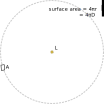
\includegraphics[width=0.5\textwidth]{figs/basics/DL_diagram.pdf}
  \end{center}
  \caption{Diagram for luminosity distance}
\end{figure}

In a static universe, the light energy collected is the same as that emitted accounting for the fraction of the area covered. So the received power at the observer is
\begin{equation}
  \frac{dE_{\rm obs}}{dt_{\rm obs}} = \frac{A}{4\pi r^2}L   \qquad \mbox{(static only)}
\end{equation}
and the observed brightness or flux (power per collecting area) is
\begin{equation}
  F = \frac{L}{4\pi r^2} =  \frac{L}{4\pi D_M^2}  \qquad \mbox{(static only)}
\end{equation}
This accounts for possible curvature but not expansion.

In an expanding universe, we have to account for two effects, both of which reduce the energy collected by the observer.  First, the rate of photons, like all rates, is slowed by the redshift factor, or equivalently $dt_{\rm obs} = (1+z) dt_{\rm em}$; it takes longer to collect the same number.  Second, the energy per photon is also redshifted, $dE_{\rm obs} = dE_{\rm em}/(1+z)$.  Accounting for these effects, we find,
\begin{equation}
    F = \frac{L}{4\pi (1+z)^2 D_M^2}.  \qquad \mbox{(correct for expansion)}
\end{equation}

Like the angular diameter distance, the luminosity distance $D_L$ is an attempt to make the expression for flux resemble the familiar relation from static, euclidean geometry:
\begin{equation}
    F = \frac{L}{4\pi D_L^2}, \label{eqn:DL}
\end{equation}
which defines $D_L$.  Although this is common, I'm once again not sure that it is such a good idea, because it seems unnecessary and confusing, as we already have the correct expression above.  On the other hand, when we are making computation about standard candles, as in Chapter \ref{ch:standard_candles}, it does make it more convenient to not have factors of (1+z) to keep track of.  In any case, the expression leads to
\begin{equation}
  D_L(z) = (1+z) D_M(z).
\end{equation}



\section*{Exercises}



\begin{enumerate}


\item Derive the expression for radial length in a spherical space, Equation (\ref{eqn:2d_sphere_path_radius}).

\item Find the analogous expression to Equation (\ref{eqn:2d_sphere_path_radius}) for  radial length in a hyperbolic space.

\item Solve the continuity equation for an equation of state $P = w\rho$ to show that $\rho \propto a^{3(1+w)}$. 

  
\item Solve the Friedmann equation to get $a(t)$ for a
  \begin{enumerate}
  \item radiation dominated universe;
  \item matter dominated universe;
  \item $\Lambda$-dominated universe.
  \end{enumerate}

\item Show that a $\Lambda$-dominated universe always has a constant Hubble parameter.

\item Show that
  \begin{equation} \frac{dt}{a(t)} = - \frac{dz}{H(z)}. \end{equation}


\item Write a compute program or make a spreadsheet that computes the comoving distance $\chi$ to redshift $z=2$ for a flat $\Lambda$CDM model with $H_0 = 70$ km/s/Mpc, $\Omega_m = 0.3$, and $\Omega_\Lambda = 0.7$.  Compute the needed integral (Equation \ref{eqn:chi_of_z}) as a Riemann sum.

  
\end{enumerate}
